\chapter{UI Design} \label{ch:ui_design}
\todo{Husk at nævn binding/WPF et eller andet sted heri}
The UI has been designed based on the model and function components and not the other way around, as the user has wished for a functional and simplistic design. This approach is more functionality oriented, than making the UI and then basing the model and function components on that.

\section{Client feedback}
As mentioned above, the ideal UI described by the client is simplistic and effective. This has resulted in an UI with few colors, cohesive design across the interface, and functionalities based on standards within the clients work environment, in this case Microsoft Windows. This is reflected in the way selections of elements in lists simply implements the Windows standard.
\par
Some things have been changed a bit from how they are handled in Windows, such as the before mentioned lists. On top of the Windows standard, checkboxes have been implemented, to make multi-select possible without holding down the control key. The client can still use the basic Windows method, but will be able to take advantage of both methods.

\subsection{Wireframes}
To ensure the compatibility between the client and the design, wireframes were developed. These has been shown to the client in the early stages of the project, to get feedback and improve the design before starting building prototypes of it.
\par
The wireframes has given a common basis for the further development of the system as well as the UI. One of the things that were illustrated in wireframes was the page with the list of all assets. This is one of the main pages of the system, as it will be used to access a specific asset, search through the assets, delete and edit assets, and print out a list of the assets. The page is very simple and is black, white, and gray (see \autoref{fig:AssetList_Wireframe}).

\begin{figure}[H]
    \centering
    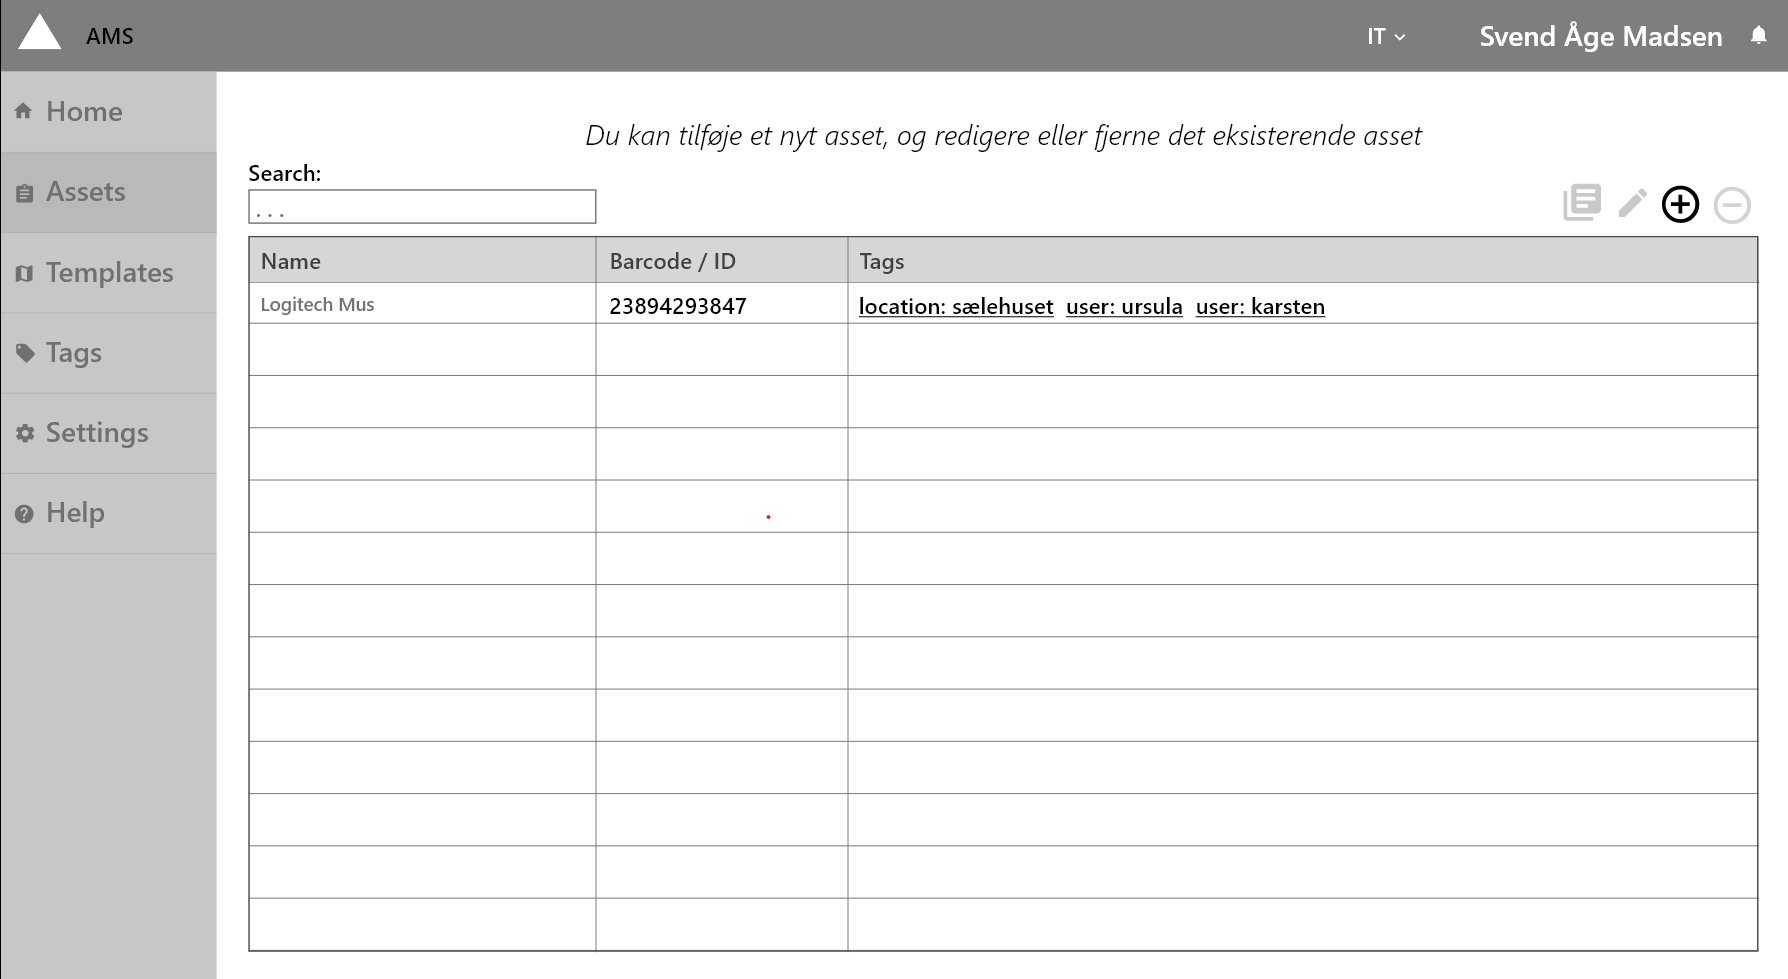
\includegraphics[width=0.8\textwidth]{figures/wireframes/AssetList_Wireframe.png}
    \caption{Wireframe of the AssetList page}
    \label{fig:AssetList_Wireframe}
\end{figure}

Another one of the essential pages was the one used for adding and editing an asset. This page has been illustrated with a few more things than the list page, as it was important to show the client how it would look after an asset had been assign a lot of things. This was important as the cluttering this could result in is the reason for the client to ask for our help, instead of going with an already existing solution. The top and side bars consist across the pages, as they contain functionalities that should be available to the user at all times. The page also contains a number of fields and attached tags, as this is another one of the specific request from the client (see \autoref{fig:AssetEditor_Wireframe}).

\begin{figure}[H]
    \centering
    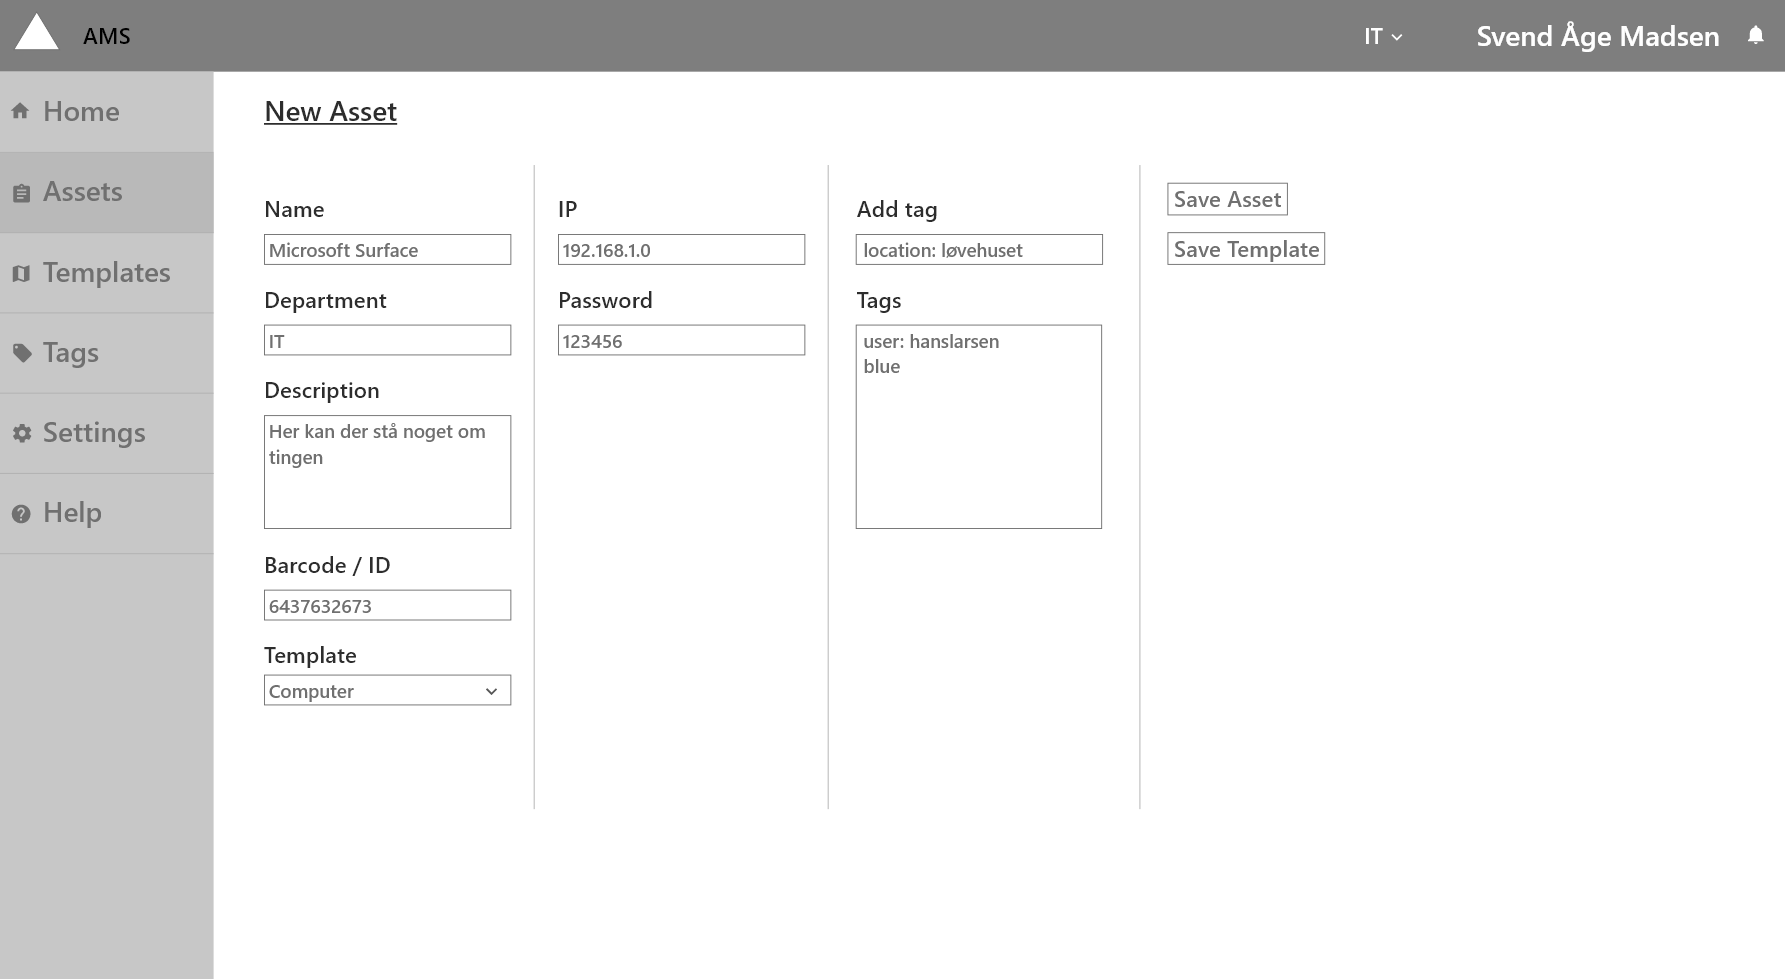
\includegraphics[width=0.8\textwidth]{figures/wireframes/AssetEditor_Wireframe.png}
    \caption{Wireframe of the AssetEditor page}
    \label{fig:AssetEditor_Wireframe}
\end{figure}

The wireframes were well received by the client, as they were very simplistic and had low saturation. The relatively few elements on the pages were also a plus for the client.

\subsection{Prototypes}
Based on the wireframes multiple prototypes were constructor to show the functionality in action. The prototypes included a the tagging of assets, which was written in Javascript (see \autoref{}), and a limited simple version of the system written in HTML, CSS, and Javascript. This method of creating prototypes made it possible to show the client the functionality in a browser. The problems with this method are that the code has to be rewritten in the used programming language, and two different programming languages might have different limitations and the implementation of certain functionalities might be more difficult in the one compared to the second.

\begin{figure}[H]
    \centering
    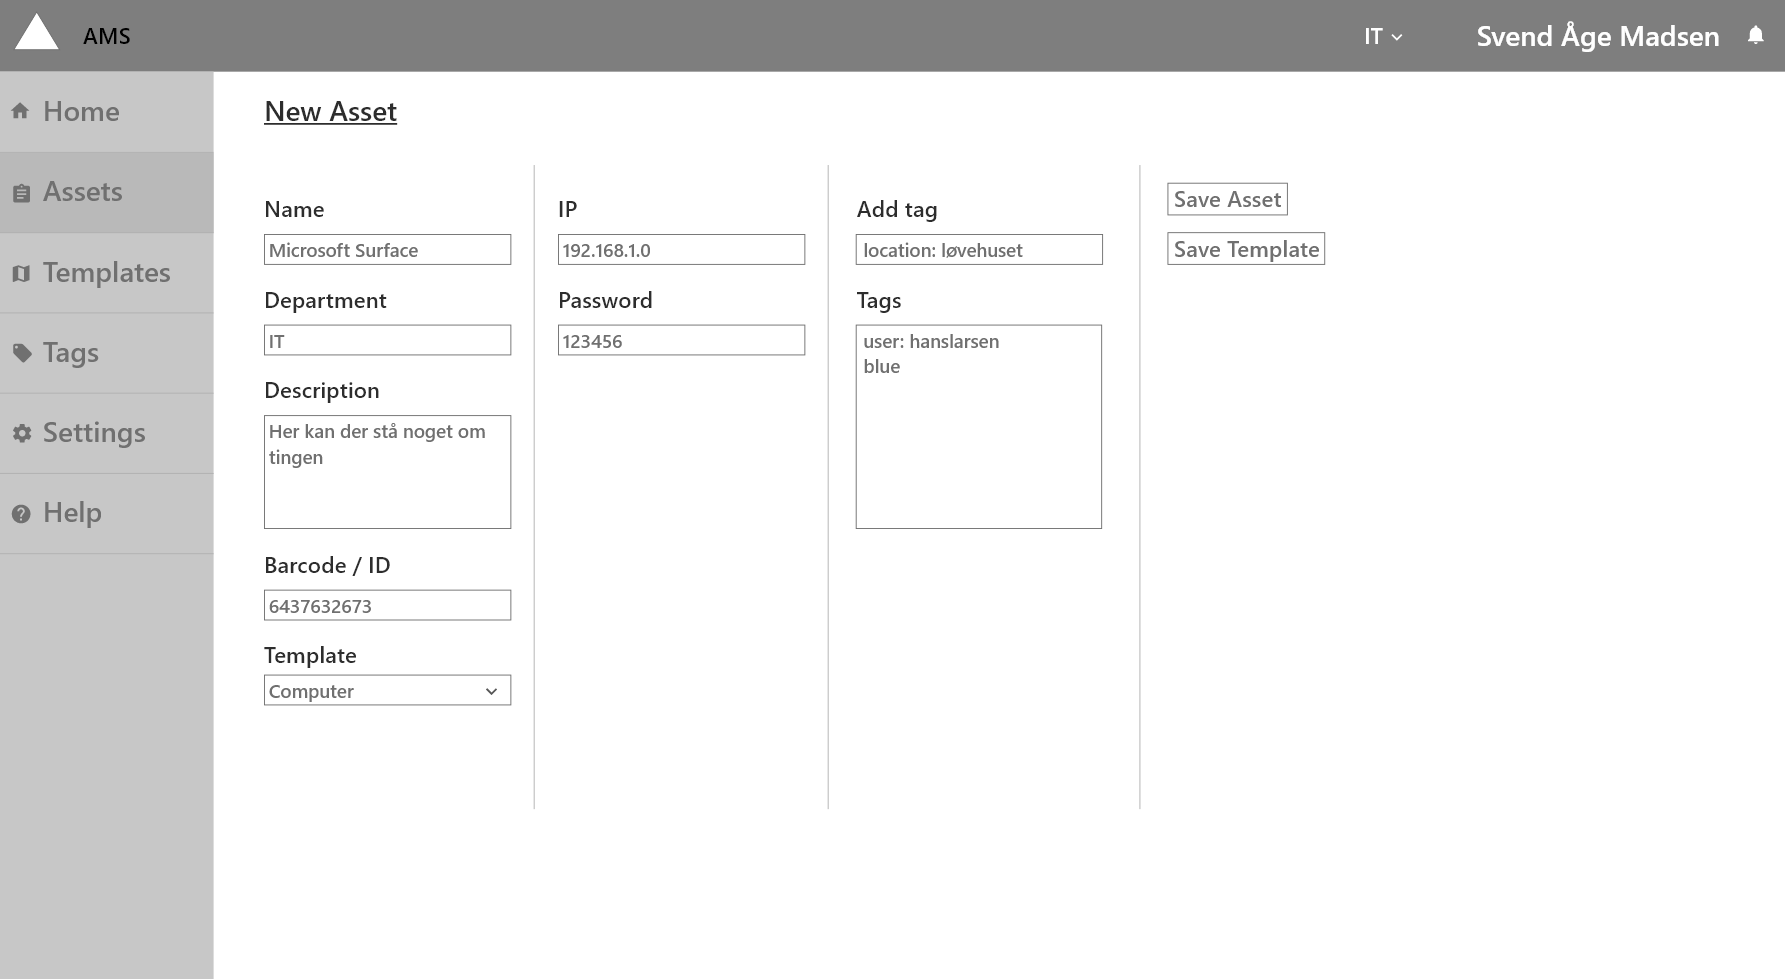
\includegraphics[width=0.8\textwidth]{figures/wireframes/AssetEditor_Wireframe.png}
    \caption{Prototype of the AssetEditor page}
    \label{fig:PrototypeOfTagging}
\end{figure}

\subsection{Early usability tests}


\section{Final design}

\subsection{Overall structure}

\subsubsection*{Navigation}

\textbf{Way finding}
% Breadcrumbs 

\subsection{Design methods}

\subsubsection*{Color}
% Colors from github and overleaf
% Button colors

\subsubsection*{Gestalt Laws}

\subsubsection*{Notifications}



% use icons!
% colors (aesthetics) 
% button positions relative to each other and the rest of the environment (Proximity)

% Gestalt laws (Proximity, continuity, similarity, closure)
    % Heuristics (System status, match between real world and digital)

% Navigation 

% Working memory

% Alerts and notifications. (ERROR, ERROR, CATASTROPHE)

% Wayfinding, breadcrumbs

% Depth perception? Layered windows, tabs. Flat design -> modern

